\chapter{Resampling Methods}
\section {Bias Variance trade off}
The Bias variance trade off is an important part of modelling and if not done right accuracy of the model will not perform well. We would like a model that that capture the structure of the data but also works well on unseen data and we can't get both. A model with high variance represent the training data well, but are at risk of overfitting hence also capturing the noise in training data. On the other hand models with high bias produce simpler models underfit their training data therefore failing to capture structure of the data.

\begin{figure}[h]
	\centering
	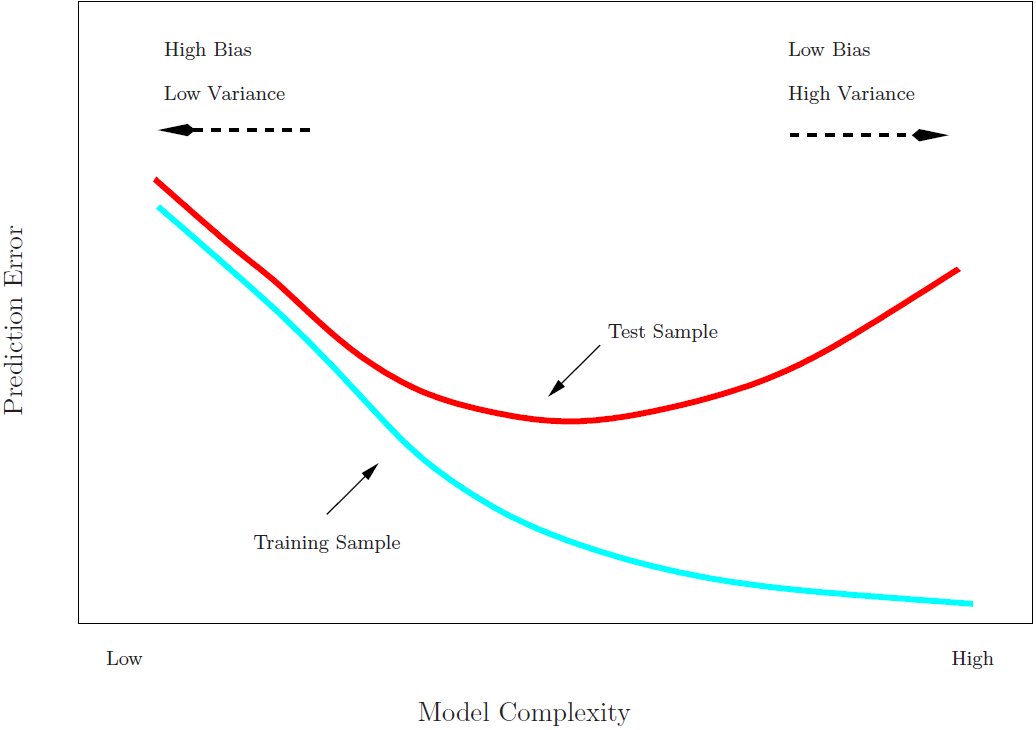
\includegraphics[width=0.5\linewidth]{crossValidation/biasVariance}
	\caption{Bias Variance trade off}
	\label{fig:biasvariance}
\end{figure}


\section{Cross Validation} \label{sc:crossValidation}
Cross validation is a technique for model validation. A model is normally trained on parts of a dataset and later another part of the dataset of unknown data will be tested against the model. With cross validation the aim is to use the the training set in the model in the training to limit problems like overfitting and help gain insight into how the model will behave to a never seen before dataset. There is several options for Cross Validation. The following sections will describe Validation set approach, Leave one out cross validation and K-fold what is the techniques used here.


\section{Validation set approach}
\subsection{Theory}
The Validation set approach works by splitting the data to two parts one is called the training set and the other is called the testing set(validation or hold-out set). An example of the split can be seen on Figure \ref{fig:validationsetapproach}. The model is trained with the training set, after the training is finished the model is tested with the testing set, which the model was not trained on. This test produces a test error, in the form of MSE, which is good for validating the model. The advantage of this method is low computation time, but the results of this method is depended on which data points will end up in the sets. 
\begin{figure}[H]
	\centering
	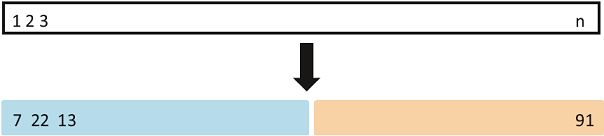
\includegraphics[width=0.4\linewidth]{crossValidation/validationSetApproach}
	\caption{Validation set approach. The entire dataset is split randomly into a training and testing set.}
	\label{fig:validationsetapproach}
\end{figure}

\subsection{Result}
\subsubsection*{LAB 5.3.1}%TODO write full lab
In lab 5.3.1\footnote{Appendix 8 - 5.3.1 The Validation Set Approach} the validation set approach is used to find estimate the test error that result from fitting linear models on the Auto data\footnote{https://raw.github.com/vincentarelbundock/Rdatasets/master/csv/ISLR/Auto.csv} set. First thing is to split the Auto dataset into a training by taking 196 random samples out of the data and use the rest for the testing. We train the model and get the following MSE
\begin{lstlisting}
23.36190289258723
\end{lstlisting}
The MSE looks high so a way to reduce the MSE could be with a polynomial 
\begin{lstlisting}[language=Python]
--------Test Error for 2nd order--------
20.25269085835005
\end{lstlisting}
Cubic regression.
\begin{lstlisting}[language=Python]
--------Test Error for 3rd order--------
20.325609365773605
\end{lstlisting}
By reviewing the results it is clear that the MSE for the models with linear, quadratic, and cubic terms are 23.36, 20.25, and 20.33.


\section {K-fold cross validation}%TODO explain in more detail (give pictures)
\subsection{Theory}
In this type of cross validation the split the data k-subsets and we repeat validation set approach for k times. In each time we take one subest as a test set and other combine are training set. After all copulations we compute average error. The advantage of this method is that all data points are one time in the testing set. The drift of the test is reduced when k is increasing. We can choose the k value, most oftenly k values are 5 or 10 . The disadvantages is that we have to retrain the model k times and the computation time increases. The mathematic formula is below. 
\begin{align}\label{fo:k-fold}
CV_{(K)} = \sum_{k=1}^{K}  \frac {n_{k}}{n}MSE_{(k)}
\end{align}

\subsection{Result}
\subsubsection*{LAB 5.3.3}%TODO write full lab
In the lab 5.3.3 we used K-fold cross validation find the MSE. We are using auto data from the book. In this particular case we are using k = 10. 
\begin{lstlisting}[language=Python]
from sklearn.model_selection import KFold

X = Data["horsepower"].values.reshape(-1,1) 
y = Data["mpg"].values.reshape(-1,1)
kf= KFold()
kf.n_splits = 10
\end{lstlisting}
Now we need to make a loop for all the folds to calculate MSE.   

\begin{lstlisting}[language=Python]
ytests = []
ypreds = []

for train_index, test_index in kf.split(Data):
	X_train, X_test = X[train_index], X[test_index]
	y_train, y_test = y[train_index], y[test_index]

	model = linear_model.LinearRegression()
	model.fit(X = X_train, y = y_train)
	y_pred = model.predict(X_test)  
	ypreds += list(y_pred)
	ytests += list(y_test)
	ms_error = metrics.mean_squared_error(ytests, ypreds)
	print("%.2f" %ms_error, end=" ")
\end{lstlisting}
Out put of the code is:
\begin{lstlisting}[language=Python]
28.35 22.79 24.14 23.95 22.29 21.56 20.92 21.16 26.11 27.42 
\end{lstlisting}
Having all MSE we can choose the best model from the results. or 
\section {Leave one out cross validation}
\subsection{Theory}
The Leave one out cross validation works a lot like Validation set approach but instead of spliting the data set into two subsets of
similar size, a single observation $(x_1, y_1)$ is used for the testing set and the remaining observations ${(x_2, y_2), . . . , (x_n, y_n)}$ make up the training set and repeat this process as seen in Figure \ref{fig:loocv}.
\begin{figure}[H]
	\centering
	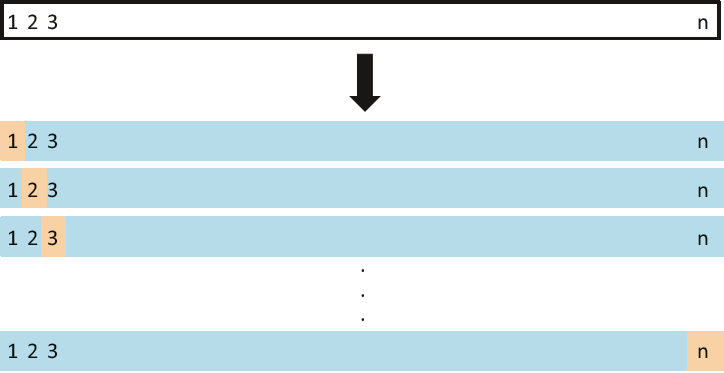
\includegraphics[width=0.5\linewidth]{crossValidation/LOOCV}
	\caption{}
	\label{fig:loocv}
\end{figure}
Repeating this method n times gives n squared errors, $MSE_1, . . . , MSE_n$. The LOOCV estimate for the test MSE is the average of these n test error as shown in Equation \ref{fo:LOOCV}.
\begin{align}\label{fo:LOOCV}
CV_{(n)} = \frac {1}{n} \sum_{k=1}^{K}  (\frac {y_i-\hat{y_i}}{1- h_i})^2
\end{align}
Leave one out cross validation has a some advantages over the validation set approach. It has far less bias. Because in LOOCV repeatedly fit the chosen learning method using training sets that contain n - 1 observations that is nearly as many as are in the entire data set. On the other hand the validation set approach training set is typically around half the size of the original data set hence LOOCV won't overestimate the test error rate as much as the validation set approach would. The LOOCV will also give consistent results because there is no randomness in the training/testing set splits and is usefull when there is limited amount of data.

\subsection{Result}
\subsubsection{LAB 5.3.2}
In lab 5.3.2 the same Auto data as used in the validation Set Approach. Running the iteratively LOOCV process for different fits polynomial regressions for polynomials of 1 to 5 and displaying the associated cross-validation error. The output below shows see a drop in the estimated test MSE between the linear and quadratic fits. But using higher-order polynomials shows no clear improvement.
\begin{lstlisting}[language=Python]
24.23151351792922, 19.24821312448969, 19.334984064109666, 19.42443031091358, 19.0332089609506
\end{lstlisting}
When running the LOOCV a mass increased computing time in the machine has seen and that was expected.
\section{Bootstrap}\label{ch:bootstrap}

A second method for producing additional information from a limited dataset is to use the bootstrap method. It is performed by shaking up the data and plucking out random observations, while allowing for the same observation to be included multiple times, to create a new sample. The process can then be repeated as many times as needed until the desired amount of data becomes available. 

\subsection{Theory}

\iffalse
A good explanation https://stats.stackexchange.com/questions/26088/explaining-to-laypeople-why-bootstrapping-works
\fi

Bootstrapping works on the assumption that distribution parameters are transitive. Such that a random number generated by taking the mean of N samples from a dataset containing N samples, but allowing for replacement, will be equally valid as a random number generated from the original population.

As an example dataset X contains N observations from the original population $\theta$ we resample from X until a new dataset Y with N elements is created. Assuming $\theta$ follows a Gaussian distribution then the mean of Y is a random number generated from the distribution of X which is an estimate of the actual distribution of $\theta$ where each observation is generated from $\theta$. Therefore the mean of Y is an estimated observation from $\theta$.

Assuming we have sufficient data then the estimated distribution can be used for generating a new, more populated, data set without sacrificing much of the quality. As the observed distribution is an estimate of the population distribution, the resulting dataset will have a distribution which is an estimate of the observations.

\iffalse % Olaf: A second attempt at writing this section. Keeping it for review purposes.
Bootstrapping works by resampling the initial data with replacement, until a new data set has been created from the original. The new dataset will then contain a random sample of data with the same distribution as the original, allowing for some deviation in the parameters. By repeating this B times and averaging the distribution parameters over all B samples we get a better estimate of the original population as if we had gotten more observations.

As an example, assuming we have a normally distributed population of N elements then by taking a random resampling from that dataset until a new dataset, also containing N elements, is gained. The mean of that new dataset can then be seen as an estimated new observation from the original population. We then repeat this process B times and in the end we have a new data set of both resampled means and variances. Since both were generated using the original set of observations the set of resamples will also be normally distributed with a mean and variance close to the original population.
\fi

To give an example of how bootstrap creates samples, see Figure \ref{fig:bootstrapDrawWithReplacement}\footnote{\cite{James2013} p. 190}. In the figure random observations are drawn from the estimated population (Original Data(Z)) with replacement. The amount of observations drawn per sample is the same amount as the observations of the estimated population. This creates bins of observations ($Z^{*1}, Z^{*2},\ldots,Z^{*B}$), from the estimated population, from which mean of the data X and Y are both calculated. The result is bootstrap samples ($\hat\alpha^{*1}, \hat\alpha^{*2}, \ldots, \hat\alpha^{*B}$).

\begin{figure}[H]
	\centering
	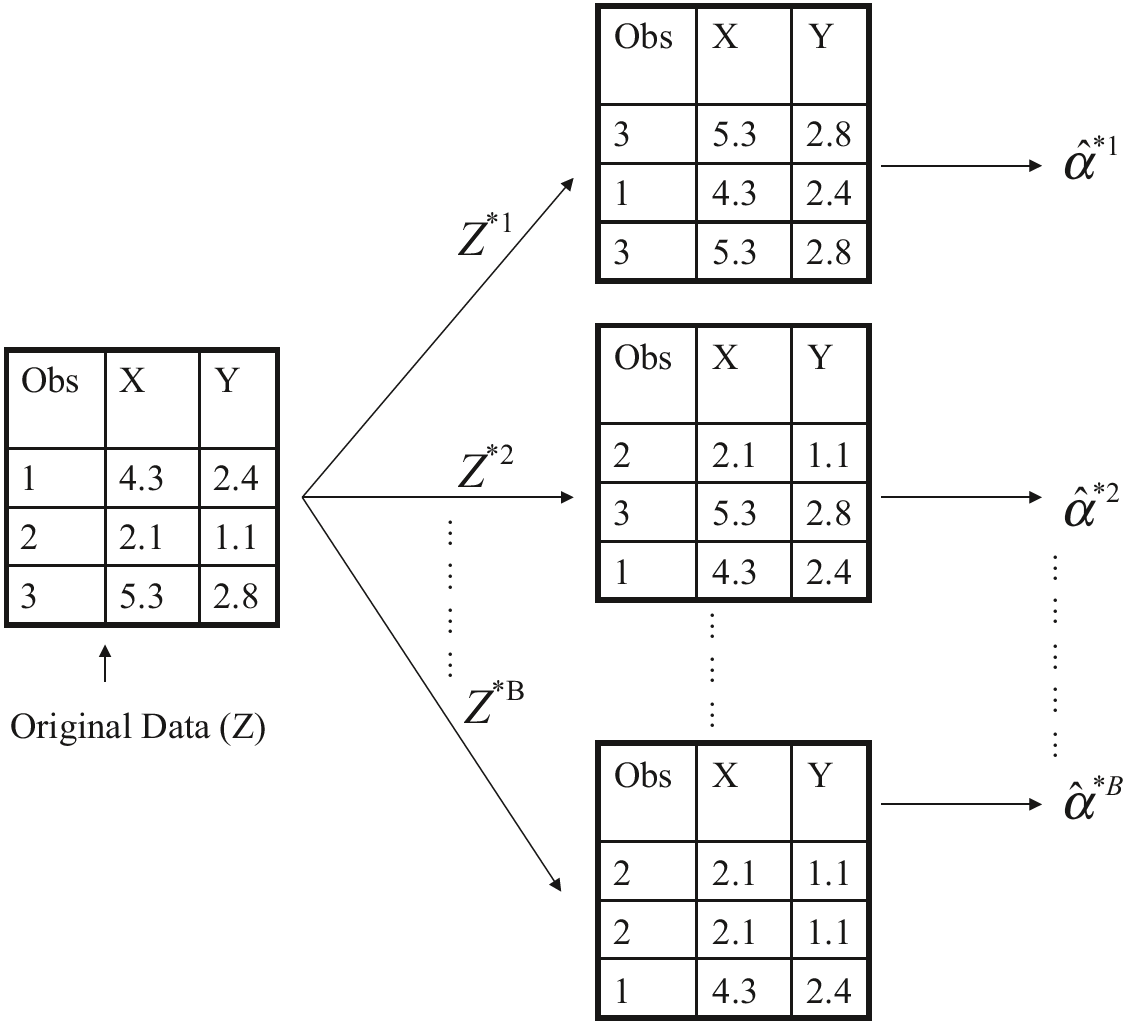
\includegraphics[width=0.5\linewidth]{crossValidation/bootstrapDrawWithReplacement}
	\caption{Bootstrap sample draw, with replacement.}
	\label{fig:bootstrapDrawWithReplacement}
\end{figure}

The standard error of the resampled data can be estimated through the sample standard deviation, as seen in Equation \ref{fo:bootstrapStandardError}. $\hat{\theta}$ denotes the bootstrap data of the estimated population $\theta$. $\hat{\theta_{b}}$ where $b=1,\dots,B$ denotes each bootstrap dataset. $\bar{\theta}$ denotes the mean of the bootstrap data; $\bar{\theta} = \frac{1}{B} \sum_{b=1}^{B}(\hat{\theta_{b}})$.
\begin{align}\label{fo:bootstrapStandardError}
	SE(\hat{\theta}) = \sqrt{\frac{1}{B-1} \sum_{b=1}^{B}(\hat{\theta_{b}} - \bar{\theta})} 
\end{align}

When working with more complex data, for example data that is not independent, but rather dependent on each other can create problems for the resampling methods of bootstrap. The solution to this problem is the Block Bootstrap alternative. Block Bootstrap does the same as the simple bootstrap mentioned earlier in this chapter, however before drawing samples from the estimated population, the data is put into smaller blocks, where the data is independent to each other. The block size is decided upon to maximize the amount of data that reside in a block, as well as minimizing the dependency between data in a single block.

\subsection{Results}
\subsubsection*{LAB 5.3.4}

In lab 5.3.4 on Bootstrap a small data sample is taken and the bootstrapping method is used to increase the data quality. First to examine the process on the Portfolio data set, and then apply the method to the auto data set and review the results for linear and quadratic regression compared to the original.

The resulting mean and error for the intercept and horsepower.
\begin{lstlisting}[language=Python]
original params
  Intercept:  mean:  39.9358610212
  Intercept:  error: 0.717498655555
  horsepower: mean:  -0.157844733354
  horsepower: error: 0.00644550051769
Bootstrapped params
  Intercept:  mean:  39.9805602832
  Intercept:  error: 0.0288069750935
  horsepower: mean:  -0.158352159577
  horsepower: error: 0.000244810973842
\end{lstlisting}

For the linear regression very similar means for both the Intercept and horsepower are found, while the RSE has dropped sharply for both the intercept and horsepower. This shows that the original estimates of the parameters were quite good as most of the error in the estimate can be explained by noise in the data and not $\epsilon_i$ as the regression formula assumes.

For the end of the exercise the same code will be run, but using a quadratic term. This time the fit to the data is very good and we see similar results as the error drops by a factor of $\sim30$.

\begin{lstlisting}[language=Python]
original params
 Intercept:  mean:               56.9000997021
 Intercept:  error:              1.80042680631
 horsepower: mean:               -0.466189629947
 horsepower: error:              0.0311246171196
 np.power(horsepower, 2): mean:  0.00123053610077
 np.power(horsepower, 2): error: 0.00012207586276
Bootstrapped params
 Intercept:  mean:               57.072651342
 Intercept:  error:              0.066630006277
 horsepower: mean:               -0.469465867184
 horsepower: error:              0.00106828698911
 np.power(horsepower, 2): mean:  0.00124365698568
 np.power(horsepower, 2): error: 3.87603834867e-06
\end{lstlisting}



